Para a criação de um tarefa de aprendizado que seja capaz de verificar a autenticidade de assinaturas de indivíduos, é necessário primeiramente a existência de um conjunto de dados de imagens que possuam exemplos de assinaturas forjadas e genuínas, com o intuito de ser utilizado para o treinamento das CNNs. Para isto, utilizou-se os conjuntos de dados disponibilizados pela Competição de Verificação de Assinaturas de 2009 (SigComp2009, do inglês \emph{Signature Verification Competition}) realizado na Conferência Internacional em Análise e Reconhecimento de Documentos (ICDAR, do inglês \emph{International Conference on Document Analysis and Recognition}).

A SigComp2009 utilizou-se de conjuntos de dados diferentes em cada uma das duas etapa da competição. Para a etapa de treinamento, foi utilizado o conjunto de assinaturas do \emph{Norwegian Information Security laboratory and Donders Centre for Cognition} (NISDCC), composto originalmente de 1.920 assinaturas genuínas e forjadas, enquanto para a etapa de validação dos modelos submetidos na competição foi aplicado o conjunto coletado pelo \emph{Netherlands Forensic Institute} (NFI), composto por 1.953 novas assinaturas genuínas e forjadas \cite{icdar2009}.

% NISDCC: Norwegian Information Security laboratory and Donders Centre for Cognition
% NFI: Netherlands Forensic Institute

O melhor tipo de falsificação de assinatura é a chamada \emph{over-the-shoulder}, na qual o autor forjador tem a oportunidade de visualizar a assinatura genuína antes da falsificação. As assinaturas forjadas encontradas nos conjuntos NISDCC e NFI pertencem a esse tipo de falsificação, nas quais os seus autores tiveram a oportunidade de praticá-las anteriormente a fim de aumentar a sua semelhança com a assinatura original. De acordo com Blankers, falsificações desse tipo normalmente são muito difíceis de detectar \cite{icdar2009}.

Os conjuntos disponibilizados pela SigComp2009 aos participantes eram compostos por dois tipos de assinaturas, as assinaturas \emph{offline} e as assinaturas \emph{online}. Nas assinaturas \emph{offline}, é considerado apenas o aspecto estático da mesma, ou seja, uma imagem obtida após o processo da assinatura ter sido concluído. Estes dados foram segmentados, inspecionados visualmente e, em seguida, pré-processados para fornecer imagens formatadas em cores, em escala de cinza e binárias com as resoluções de 300 e 600 dpi. Os dados das assinaturas \emph{online}, por sua vez, continham informações dinâmicas, que consistiam em arquivos de texto que descreviam os detalhes capturados em vários pontos durante o processo da assinatura, sendo estes as coordenadas $x$ e $y$ da ponta da caneta, a pressão exercida sobre a caneta, o ângulo de azimute e o ângulo de elevação \cite{icdar2009}. Um exemplo de uma assinatura \emph{offline} e a sua representação \emph{online} com os pontos plotados pode ser encontrada na Figura \ref{fig:sample-signature}.


\begin{figure}[h!]
\centering
\caption{Uma amostra das assinaturas \emph{offline} e \emph{online}. Fonte: \cite{icdar2009}}
\label{fig:sample-signature}
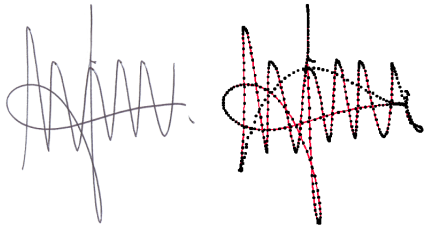
\includegraphics[width=0.5\textwidth]{imgs/sample-signature}
\end{figure}

Apesar da quantidade de assinaturas originalmente utilizada na competição, foram disponibilizadas atráves da \emph{International Association for Pattern Recognition} (IAPR) apenas 1.898 assinaturas do conjunto NISDCC e 1.564 assinaturas do conjunto NFI \cite{iapr-tc11}. Desses dados disponibilizados, apenas as assinaturas \emph{offline} de cada conjunto foram utilizadas para a construção dos modelos propostos para a resolução do problema descrito neste trabalho, devido a preferência por desenvolver uma solução em visão computacional. Uma demonstração dos dados disponibilizados pela IAPR em relação a quantidade de autores e assinaturas pode ser visualizado na Tabela \ref{tab:demonstracao-dataset}.

\begin{table}[h!]
	\centering
	\caption{Quantitativo de indivíduos e assinaturas por conjunto de dados.}
	\label{tab:demonstracao-dataset}
\resizebox{\textwidth}{!}{
	\begin{tabular}{c C{2cm} C{2cm} C{3.25cm} C{2.5cm} C{2.5cm} C{2.25cm}}
		\toprule
		 \textbf{Conjunto}& \textbf{Autores originais} & \textbf{Autores forjadores} & \textbf{Autores originais com assinaturas forjadas} & \textbf{Assinaturas genuínas}  & \textbf{Assinaturas forjadas} & \textbf{Total de assinaturas} \\
		\midrule
		NISDCC & 12 & 31 & 12 & 60 & 1.838 & 1.898 \\
    NFI & 79 & 33 & 19 & 940 & 624 & 1.564 \\
		\bottomrule
	\end{tabular}}
\end{table}

As imagens correspondentes às assinaturas \emph{offline} presentes nos conjuntos estão em formato \emph{png}, com resolução de 600 dpi e com diferentes dimensões, de forma que todo o conteúdo da assinatura em questão seja visualizado. Contudo, a fim de padronizar esta base de dados para a criação de exemplos compatíveis com o modelo que deseja-se desenvolver, é necessário um pré-processamento das suas imagens, conforme descrito na seção a seguir.



% Conjuntos de treino e validação disponibilizados pela competição (NISDCC e NFI)
% Assinaturas online e offline
% Como foram feitas as assinaturas forjadas
% A quantidade de indivíduos no dataset
% A quantidade de assinaturas por indivíduo
